\chapter{Аналитический раздел}
\label{cha:analysis}

DES является блочным шифром. Чтобы понять, как работает DES, необходимо рассмотреть принцип работы блочного шифра, сеть Фейстеля.
\section{Блочный шифр}

Входными данными для блочного шифра служат:
\begin{itemize}
    \item блок размером n бит;
    \item ключ размером k бит.
\end{itemize}

На выходе (после применения шифрующих преобразований) получается зашифрованный блок размером n бит, причём незначительные различия входных данных, как правило, приводят к существенному изменению результата.

Блочные шифры реализуются путём многократного применения к блокам исходного текста некоторых базовых преобразований.

Базовые преобразования:
\begin{itemize}
    \item сложное преобразование на одной локальной части блока;
    \item простое преобразование между частями блока.
\end{itemize}

Так как преобразования производятся поблочно, требуется разделение исходных данных на блоки необходимого размера. При этом формат исходных данных не имеет значения (будь то текстовые документы, изображения или другие файлы). Данные должны интерпретироваться в двоичном виде (как последовательность нулей и единиц) и только после этого должны разбиваться на блоки. Все вышеперечисленное может осуществляться как программными, так и аппаратными средствами.

\section{Преобразования Сетью Фейстеля}
Это преобразование над векторами (блоками), представляющими собой левую и правую половины регистра сдвига. В алгоритме DES используются прямое преобразование сетью Фейстеля в шифровании (см. Рисунок 1.1) и обратное преобразование сетью Фейстеля в расшифровании (см. Рисунок 1.2).
\begin{figure}[H]
\centering
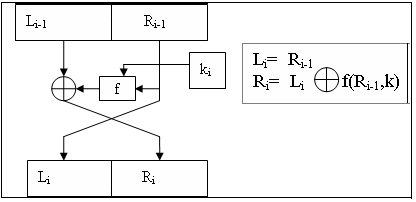
\includegraphics[scale=1.5]{pict/netF1.png}
\caption{Прямое преобразование сетью Фейстеля}
\end{figure}

\begin{figure}[H]
\centering
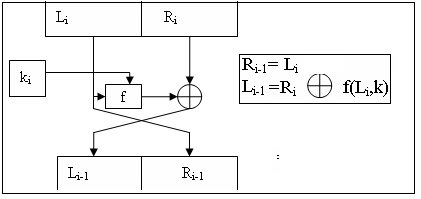
\includegraphics[scale=1.5]{pict/netF2.png}
\caption{Обратное преобразование сетью Фейстеля}
\end{figure}

\section{Схема шифрования алгоритма DES}
Схема шифрования алгоритма DES указана на Рисунке 1.3.
\begin{figure}[H]
\centering
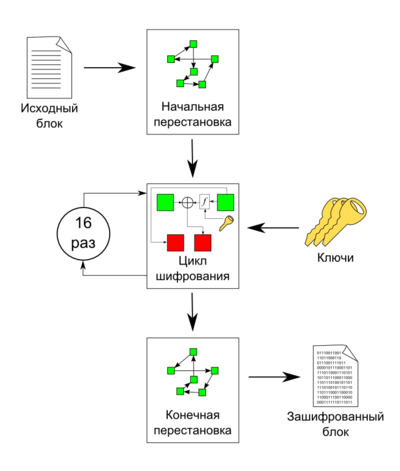
\includegraphics[scale=0.85]{pict/DES_algorithm_scheme.png}
\caption{Схема шифрования алгоритма DES}
\end{figure}

Исходный текст — блок 64 бит.

Процесс шифрования состоит из начальной перестановки, 16 циклов шифрования и конечной перестановки.

\subsection{Начальная перестановка}
Исходный текст \textbf{T} (блок 64 бит) преобразуется c помощью начальной перестановки \textbf{IP} которая определяется таблицей 1:
\begin{table}[H]
    \caption{Начальная перестанвока IP}
	\begin{tabular}{|c|c|c|c|c|c|c|c|c|c|c|c|c|c|c|c|}
    \hline
    58 & 50 & 42 & 34 & 26 & 18 & 10 & 2 & 60 & 52 & 44 & 36 & 28 & 20 & 12 & 4\\
    \hline
    62 &	54 &	46 &	38 &	30 &	22 &	14 &	6 &	64 &	56 &	48 &	40 &	32 &	24 &	16 &	8\\
    \hline
    57 &	49 &	41 &	33 &	25 &	17 &	9 &	1 &	59 &	51 &	43 &	35 &	27 &	19 &	11 &	3\\
    \hline
    61 &	53 &	45 &	37 &	29 &	21 &	13 &	5 &	63 &	55 &	47 &	39 &	31 &	23 &	15 &	7\\
    \hline
	\end{tabular}
\end{table}
По таблице первые 3 бита результирующего блока \textbf{IP(T)} после начальной перестановки \textbf{IP} являются битами 58, 50, 42 входного блока \textbf{T}, а его 3 последние бита являются битами 23, 15, 7 входного блока.

\subsection{Циклы шифрования}

Полученный после начальной перестановки 64-битовый блок IP(T) участвует в 16 циклах преобразования Фейстеля.

— 16 циклов преобразования Фейстеля:

Разбить IP(T) на две части $L_0,R_0$, где $L_0, R_0$ — соответственно 32 старших битов и 32 младших битов блока $T_0$ IP(T)= $L_0R_0$

Пусть $T_{i-1} = L_{i-1}R_{i-1}$ результат (i-1) итерации, тогда результат i-ой итерации $T_{i}=L_{i}R_{i}$ определяется:
\[L_{i}=R_{i-1}\]
\[R_{i}=L_{i-1}\oplus f(R_{i-1},k_{i})\]
Левая половина $L_{i}$ равна правой половине предыдущего вектора $L_{i-1}R_{i-1}$. А правая половина $R_{i}$ — это битовое сложение $L_{i-1}$ и $f(R_{i-1},k_{i})$ по модулю 2.

В 16-циклах преобразования Фейстеля функция f играет роль шифрования. Рассмотрим подробно функцию f.

\subsection{Основная функция шифрования (функция Фейстеля)}

Аргументами функции $f$ являются 32-битовый вектор $R_{i-1}$ и 48-битовый ключ $k_{i}$, который является результатом преобразования 56-битового исходного ключа шифра $k$. Для вычисления функции $f$ последовательно используются:
\begin{enumerate}
    \item функция расширения $E$,
    \item сложение по модулю 2 с ключом $k_i$
    \item преобразование $S$, состоящее из 8 преобразований $S$-блоков $S_{1}, S_{2}, S_{3 }\ldots S_8$,
    \item перестановка $P$.
\end{enumerate}

Функция $E$ расширяет 32-битовый вектор $R_{i-1}$ до 48-битового вектора $E(R_{i-1})$ путём дублирования некоторых битов из $R_{i-1}$; порядок битов вектора $E(R_{i-1})$ указан в таблице 2.
\begin{table}[H]
    \caption{Функция расширения E}
	\begin{tabular}{|c|c|c|c|c|c|}
    \hline
    32	& 1	& 2	& 3	& 4	& 5\\
    \hline
    4	& 5	& 6	& 7	& 8	& 9\\
    \hline
    8	& 9	& 10	& 11	& 12	& 13\\
    \hline
    12	& 13	& 14	& 15	& 16	& 17\\
    \hline
    16	& 17	& 18	& 19	& 20	& 21\\
    \hline
    20	& 21 &	22	& 23	& 24	& 25\\
    \hline
    24	& 25	& 26	& 27	& 28	& 29\\
    \hline
    28	& 29	& 30	& 31	& 32	& 1\\
    \hline
	\end{tabular}
\end{table}

Первые три бита вектора $E(R_{i-1})$ являются битами 32, 1, 2 вектора $R_{i-1}$. По таблице 2 видно, что биты 1, 4, 5, 8, 9, 12, 13, 16, 17, 20, 21, 24, 25, 28, 29, 32 дублируются. Последние 3 бита вектора $E(R_{i-1})$ — это биты 31, 32, 1 вектора $R_{i-1}$. Полученный после перестановки блок $E(R_{i-1})$ складывается по модулю 2 с ключами $k_i$ и затем представляется в виде восьми последовательных блоков $B_{1},B_{2},...B_{8}$.

\[E(R_{i-1})\oplus k_{i}=B_{1}B_{2}...B_{8}\]
Каждый $B_j$ является 6-битовым блоком. Далее каждый из блоков $B_j$ трансформируется в 4-битовый блок $B'_j$ с помощью преобразований $S_j$. Преобразования $S_j$ определяются на рисунке 1.4.

\begin{figure}[H]
\centering
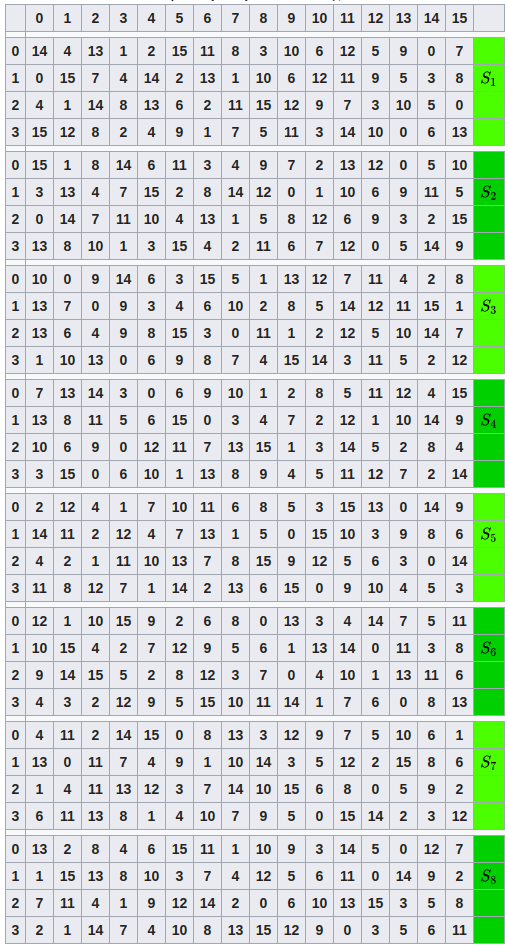
\includegraphics[scale=0.7]{pict/table.png}
\caption{Таблица 3. Преобразования $S_{i}, i=1…8$}
\end{figure}

Предположим, что $B_3 = 101111$, и мы хотим найти $B'_3$. Первый и последний разряды $B_{3}$ являются двоичной записью числа а, 0<=a<=3, средние 4 разряда представляют число b, 0<=b<=15. Строки таблицы S3 нумеруются от 0 до 3, столбцы таблицы S3 нумеруются от 0 до 15. Пара чисел (а, b) определяет число, находящееся в пересечении строки а и столбца b. Двоичное представление этого числа дает $B'_3$ . В нашем случае $a=11_{2}=3$, $b=0111_{2}=7$, а число, определяемое парой (3,7), равно 7. Его двоичное представление $B'_{3}$. Значение функции $f(R_{i-1},k_{i})$ (32 бит) получается перестановкой Р, применяемой к 32-битовому блоку $B'_{1}B'_{2}...B'_{8}$. Перестановка Р задана таблицей 3.

\begin{table}[H]
    \caption{Перестановка P}
	\begin{tabular}{|c|c|c|c|c|c|c|c|}
    \hline
    16	& 7	& 20	& 21	& 29	& 12	& 28	& 17\\
    \hline
    1	& 15	& 23	& 26	& 5	& 18	& 31	& 10\\
    \hline
    2	& 8	& 24	& 14	& 32	& 27	& 3	& 9\\
    \hline
    19	& 13	& 30	& 6	& 22	& 11	& 4	& 25\\
    \hline
	\end{tabular}
\end{table}

\[f(R_{i-1},k_i) = P(B'_1B'_2...B'_8)\]
Согласно таблице 4, первые четыре бита результирующего вектора после действия функции f — это биты 16, 7, 20, 21 вектора $B'_{1}B'_{2}...B'_{8}$

\subsection{Генерирование ключей $k_i$}

Ключи $k_i$ получаются из начального ключа $k$ (56 бит = 7 байтов или 7 символов в ASCII) следующим образом. Добавляются биты в позиции 8, 16, 24, 32, 40, 48, 56, 64 ключа $k$ таким образом, чтобы каждый байт содержал нечетное число единиц. Это используется для обнаружения ошибок при обмене и хранении ключей. Затем делают перестановку для расширенного ключа (кроме добавляемых битов 8, 16, 24, 32, 40, 48, 56, 64). Такая перестановка определена в таблице 4.
\begin{table}[H]
    \caption{Перестановка P}
	\begin{tabular}{|c|c|c|c|c|c|c|c|c|c|c|c|c|c|c|}
    \hline
    57	& 49	& 41	& 33	& 25	& 17	& 9	& 1	& 58	& 50	& 42	& 34	& 26	& 18 &	$C_{0}$\\
    \hline
    10	& 2	& 59	& 51	& 43	& 35	& 27	& 19	& 11	& 3	& 60	& 52	& 44	& 36 &\\
    \hline
    63	& 55	& 47	& 39	& 31	& 23	& 15	& 7	& 62 &	54	& 46	& 38	& 30	& 22 & $D_0$\\
    \hline
    14	& 6	& 61	& 53	& 45	& 37	& 29	& 21	& 13	& 5	& 28	& 20	& 12	& 4&\\
    \hline
    \end{tabular}
\end{table}

Эта перестановка определяется двумя блоками $C_{0}$ и $D_0$ по 28 бит каждый. Первые 3 бита $C_{0}$ есть биты 57, 49, 41 расширенного ключа. А первые три бита $D_0$ есть биты 63, 55, 47 расширенного ключа. $C_i, D_i i=1,2,3… $получаются из $C_{i-1}, D_{i-1}$ одним или двумя левыми циклическими сдвигами согласно таблице 5.
\begin{table}[H]
    \caption{}
	\begin{tabular}{|c|c|c|c|c|c|c|c|c|c|c|c|c|c|c|c|c|}
    \hline
    i	& 1	& 2	& 3	& 4	& 5	& 6	& 7	& 8	& 9	& 10	& 11	& 12	& 13	& 14	& 15	& 16\\
    \hline
    Число сдвига	& 1	& 1	& 2	& 2	& 2	& 2	& 2	& 2	& 1	& 2	& 2	& 2	& 2	& 2	& 2 &	1\\
    \hline
    \end{tabular}
\end{table}

Ключ $k_i$, i=1,…16 состоит из 48 бит, выбранных из битов вектора $C_{i}D_{i}$ (56 бит) согласно таблице 7. Первый и второй биты $k_i$ есть биты 14, 17 вектора $C_{i}D_{i}$

\begin{table}[H]
    \caption{}
	\begin{tabular}{|c|c|c|c|c|c|c|c|c|c|c|c|c|c|c|c|}
	\hline
	14	& 17	& 11	& 24	& 1	& 5	& 3	& 28	& 15	& 6	& 21	& 10	& 23	& 19	& 12	& 4\\
	\hline
	26	& 8	& 16	& 7	& 27	& 20	& 13 &	2	& 41	& 52	& 31	& 37	& 47	& 55	& 30	& 40\\
	\hline
	51	& 45	& 33	& 48	& 44	& 49	& 39	& 56	& 34	& 53	& 46	& 42	& 50	& 36	& 29	& 32\\
	\hline
	\end{tabular}
\end{table}

\subsection{Конечная перестановка}
Конечная перестановка $IP^{-1}$ действует на $T_{16}$ и является обратной к первоначальной перестановке. Конечная перестановка определяется таблицей 1.7.
\begin{table}[H]
	\caption{}
	\begin{tabular}{|c|c|c|c|c|c|c|c|c|c|c|c|c|c|c|c|}
	\hline
	40  & 8  & 48 & 16 & 56 & 24 & 64 & 32 & 39 & 7 &  47 & 15 & 55 & 23 & 63 & 31\\
	\hline
	38 & 6  & 46 & 14 & 54 & 22 & 62 & 30 & 37 & 5  & 45 & 13 & 53 & 21 & 61 & 29\\
	\hline
	36 & 4  & 44 & 12 & 52 & 20 & 60 & 28 & 35 & 3  & 43 & 11 & 51 & 19 & 59 & 27\\
	\hline
	34 & 2  & 42 & 10 & 50 & 18 & 58 & 26 & 33 & 1  & 41 & 9  & 49 & 17 & 57 & 25\\
	\hline
	\end{tabular}
\end{table}
